\documentclass{beamer}
%\documentclass[handout]{beamer}
%\usepackage{xeCJK}

\usepackage{ctex}
 % 1. packages

 % ----------- fonts and symbles ---------
\usepackage{amsmath,amssymb,amsfonts,amsthm}
%\usepackage{CJK}
\usepackage{dsfont}
\usepackage{mathrsfs}
\usepackage{eucal} % for \mathcal

%\renewcommand{\rmdefault}{ptm}


%\usepackage{fontspec}
%\newfontfamily\monaco{Monaco}

%\usepackage{mathbbold} %,bbold

 \usepackage{textcomp} % for \textnormal{\textperthousand}
% -----------------





%\usepackage{slashbox}
%\usepackage[margin=2.2cm]{geometry} % |geometry| package clash with |booktabs| package
%\usepackage{cases}
% -------- tables -------
\usepackage{booktabs} % for \toprule, \bottomrule
\usepackage{tabularx}
\usepackage{multirow}
% --------- figures ---------
\usepackage{graphicx}
% ---------- algorithms -------
\usepackage{algorithm}
\usepackage{algorithmic}
%\usepackage{footnote}
    % |footnote| package occurs error:
    % Runaway argument?
    % \def \insertfootnotetext {\@@ }\def \insertfootnotemark {\@makefnmark \ETC.

\usepackage{listings}

\usepackage[linewidth=1pt]{mdframed} % for  mdframe environment




 \usepackage{color}
 \usepackage{xcolor}     %¸ßÁÁʹÓõÄÑÕÉ«

\usepackage{setspace}
%%\usepackage{type1cm}
\usepackage{adjustbox} % for \adjustbox

\usepackage{accsupp}
\newcommand{\emptyaccsupp}[1]{\BeginAccSupp{ActualText={}}#1\EndAccSupp{}}




%%   figures and tables
\graphicspath{{figure/}}


% 2. new commands

% 2.0 common commands
%\newcommand{\bc}{\begin{center}}
%\newcommand{\ec}{\end{center}}
%\newcommand{\ba}{\begin{array}}
%\newcommand{\ea}{\end{array}}
%\newcommand{\be}{\begin{equation}}
%\newcommand{\ee}{\end{equation}}

% 2.1 colors
\definecolor{dgrey}{rgb}{0.30,0.30,0.30}
\definecolor{lred}{rgb}{0.50,0.00,0.50}
\definecolor{lblue}{rgb}{0.8,0.8,1}
\definecolor{dred}{rgb}{0.6,0,0}
\definecolor{dblue}{rgb}{0,0,0.5}
\definecolor{dgrey}{rgb}{0.35,0.35,0.35}
\definecolor{rred}{rgb}{0.9,0,0}
\definecolor{mylblue}{rgb}{0.3,0.2, 0.8}

\definecolor{commentcolor}{RGB}{85,139,78}
\definecolor{stringcolor}{RGB}{206,145,108}
\definecolor{keywordcolor}{RGB}{34,34,250}
\definecolor{backcolor}{RGB}{220,220,220}

\newcommand{\blue}[1]{{\color{blue}#1}}
\newcommand{\dblue}[1]{{\color{dblue}#1} }
\newcommand{\red}[1]{{\color{red}#1}}
\newcommand{\dred}[1]{{\color{dred}#1}}
\newcommand{\cyan}[1]{{\color{cyan}#1}}
\newcommand{\bfblue}[1]{\textbf{\color{dblue}#1} }
\newcommand{\bfred}[1]{\textbf{\color{dred}#1} }
\newcommand{\green}[1]{{\color{green}#1}}
%\newcommand{\alert}[1]{{\color{red}#1}}
\newcommand{\black}[1]{{\color{black}#1}}
\newcommand{\light}[1]{{\color{blue}\textbf{#1}}}
\newcommand{\hot}[1]{{\color{dred}#1}}
 \newcommand{\highlight}[1]{ \textbf{\color{mylblue}#1}}
 \newcommand{\important}[1]{{\color{red}#1}} % for highlighting  some words

 \newcommand{\mystar}{\dred{$^{\clubsuit}$ }}
  \newcommand{\doublestar}{\dred{$^{\clubsuit\clubsuit}$ }}

\newcommand{\mynote}[1]{{\footnotesize \color{mylblue}#1}}

 \newcommand{\hint}[1]{{\small \color{mylblue}#1}}
\newcommand{\smallhint}[1]{{\small \color{dgrey}#1}}
\newcommand{\footnotehint}[1]{{\footnotesize \color{dgrey}#1}}
\newcommand{\tinyhint}[1]{{\tiny \color{dgrey}#1}}
\newcommand{\mytitle}[1]{\medskip{\large \textbf{\color{mylblue}#1}}}
\newcommand{\normaltitle}[1]{\medskip{ \textbf{\color{mylblue}#1}}}

%\newcommand{\head}[1]{\textbf{\large\color{blue}#1}}
%\newcommand{\heading}[1]{\textbf{\large\color{blue}#1}}

\newcommand{\myfbox}[2]{ \bigskip \begin{center} \fbox{\parbox{#1}{ #2  }} \end{center}\bigskip }

\newcommand{\myvar}[1]{}
%\newcommand{\mynote}[1]{#1}

% 2.2 mathematical symbols

\newcommand{\drightarrow}{\stackrel{d.}{\rightarrow}}
\newcommand{\prightarrow}{\stackrel{p.}{\rightarrow}}
\newcommand{\bernoulli}{\textnormal{Ber}}
\newcommand{\cov}{\mathsf{Cov}}
\newcommand{\corr}{\mathbf{Corr}}
\newcommand{\regret}{\textnormal{Regret}}
\newcommand{\conv}{\textnormal{conv}}
\newcommand{\dotdiv}{\stackrel{\centerdot}{-}}
\newcommand{\dom}{\textnormal{dom}}
\newcommand{\convergenceinprob}{\stackrel{P}{\rightarrow}}
\newcommand{\convergenceindist}{\rightsquigarrow}
\newcommand{\probability}{\mathbb{P}}
\newcommand{\expectation}{\mathbb{E}}
\newcommand{\epi}{\textnormal{epi}}
\newcommand{\variance}{\mathbb{V}}
\newcommand{\var}[1]{\mathbb{V}(#1)}
\newcommand{\covariance}{\mathsf{Cov}}
\newcommand{\empiricalrisk}[1]{\hat{R}(#1)}
\newcommand{\expectedrisk}[1]{R(#1)}
\newcommand{\mgf}[1]{\psi_{#1}(\lambda)}
\newcommand{\mgfexpansion}[1]{\expectation[e^{\lambda#1}]}
\newcommand{\mgfmultivariate}[1]{\expectation[e^{\lambda^\transpose#1}]}
\newcommand{\transpose}{{\mathsf{T}}}
\newcommand{\real}{\mathbb{R}}
\newcommand{\gaussian}[2]{\mathcal{N}(#1,#2)}
\newcommand{\subGaussian}[1]{\mathsf{subG}(#1)}
\newcommand{\indicator}[1]{\mathbb{I}[#1]}
\newcommand{\x}[1]{x^{(#1)}}
\newcommand{\y}[1]{y^{(#1)}}
\newcommand{\z}[1]{z^{(#1)}}
\newcommand{\feature}{x}
\newcommand{\response}{y}
\newcommand{\supofempiricalprocess}{\|\mathbb{P}_n-\mathbb{P}\|_{\decisionspace}}
\newcommand{\decisionspace}{\mathscr{F}}
\newcommand{\decisionfunction}{f}
\newcommand{\featurespace}{\mathcal{X}}
\newcommand{\classifierestimate}{\widehat{h}}
\newcommand{\classifiertrue}{h^\star}
\newcommand{\classifier}{h}
\newcommand{\hypothesisclass}{\mathcal{H}}
\newcommand{\dataset}{\mathcal{D}}
\newcommand{\defineas}{\stackrel{\textnormal{def}}{=}}
\newcommand{\rademachercomplexity}[1]{\mathsf{Rad}_n\left(#1\right)}
\newcommand{\loss}{\ell}
\newcommand{\composite}{\circ}
\newcommand{\convexhull}{\mathsf{conv}}
\newcommand{\norm}[2][2]{\|#2\|_{#1}}
\newcommand{\shatteringcoefficient}[2]{\mathcal{S}(#1,#2)}
\newcommand{\vcdimension}[1]{\mathsf{VC}\left(#1\right)}
\newcommand{\rank}{\mathsf{rank}}
\newcommand{\innerproduct}[2]{\left\langle #1, #2\right\rangle}
\newcommand{\modelparameter}{\theta}
\newcommand{\ball}[3][]{\mathcal{B}_{{#1}}\left(#2,#3\right)}
\newcommand{\metric}{d}
\newcommand{\coveringnumber}[4][]{N_{{#1}}\left(#2,#3,#4\right)}
\newcommand{\trace}{\textnormal{tr}}
\newcommand{\std}{\textnormal{std}}
\newcommand{\sgn}{\textnormal{sign}}
%\renewcommand{\span}{\textnormal{span}}

 % do not overwrite the existing command \span
 % as it leads to an error of
 %  "Missing # Inserted in Alignment Preamble" for ``align'' environment

\newcommand{\myspan}{\textnormal{span}}

%%%
\newcommand{\rightarrowd}{\stackrel{d}{\rightarrow}}
\newcommand{\rightarrowp}{\stackrel{p}{\rightarrow}}
\newcommand{\defeq}{ \stackrel{\textnormal{def}}{=}}
\newcommand{\proj}{ \textnormal{Proj}}
\newcommand{\dist}{\textnormal{dist}}

\newcommand{\argmax}{\textnormal{argmax}}
\newcommand{\argmin}{\textnormal{argmin}}
\newcommand{\subg}{\textnormal{subG}}


 \newcommand{\bba}{\mathbb{A}}
\newcommand{\bbb}{\mathbb{B}}
\newcommand{\bbc}{\mathbb{C}}
\newcommand{\bbd}{\mathbb{D}}
\newcommand{\bbe}{\mathbb{E}}
\newcommand{\bbf}{\mathbb{F}}
\newcommand{\bbg}{\mathbb{G}}
\newcommand{\bbh}{\mathbb{H}}
\newcommand{\bbi}{\mathbb{I}}
\newcommand{\bbj}{\mathbb{J}}
\newcommand{\bbk}{\mathbb{K}}
\newcommand{\bbl}{\mathbb{L}}
\newcommand{\bbm}{\mathbb{M}}
\newcommand{\bbn}{\mathbb{N}}
\newcommand{\bbo}{\mathbb{O}}
\newcommand{\bbp}{\mathbb{P}}
\newcommand{\bbq}{\mathbb{Q}}
\newcommand{\bbr}{\mathbb{R}}
\newcommand{\bbs}{\mathbb{S}}
\newcommand{\bbt}{\mathbb{T}}
\newcommand{\bbu}{\mathbb{U}}
\newcommand{\bbv}{\mathbb{V}}
\newcommand{\bbw}{\mathbb{W}}
\newcommand{\bbx}{\mathbb{X}}
\newcommand{\bby}{\mathbb{Y}}
\newcommand{\bbz}{\mathbb{Z}}

\newcommand{\bfa}{\mathbf{a}}
\newcommand{\bfb}{\mathbf{b}}
\newcommand{\bfc}{\mathbf{c}}
\newcommand{\bfd}{\mathbf{d}}
\newcommand{\bfe}{\mathbf{e}}
\newcommand{\bff}{\mathbf{f}}
\newcommand{\bfg}{\mathbf{g}}
\newcommand{\bfh}{\mathbf{h}}
\newcommand{\bfi}{\mathbf{i}}
\newcommand{\bfj}{\mathbf{j}}
\newcommand{\bfk}{\mathbf{k}}
\newcommand{\bfl}{\mathbf{l}}
\newcommand{\bfm}{\mathbf{m}}
\newcommand{\bfn}{\mathbf{n}}
\newcommand{\bfo}{\mathbf{o}}
\newcommand{\bfp}{\mathbf{p}}
\newcommand{\bfq}{\mathbf{q}}
\newcommand{\bfr}{\mathbf{r}}
\newcommand{\bfs}{\mathbf{s}}
\newcommand{\bft}{\mathbf{t}}
\newcommand{\bfu}{\mathbf{u}}
\newcommand{\bfv}{\mathbf{v}}
\newcommand{\bfw}{\mathbf{w}}
\newcommand{\bfx}{\mathbf{x}}
\newcommand{\bfy}{\mathbf{y}}
\newcommand{\bfz}{\mathbf{z}}

\newcommand{\bfA}{\mathbf{A}}
\newcommand{\bfB}{\mathbf{B}}
\newcommand{\bfC}{\mathbf{C}}
\newcommand{\bfD}{\mathbf{D}}
\newcommand{\bfE}{\mathbf{E}}
\newcommand{\bfF}{\mathbf{F}}
\newcommand{\bfG}{\mathbf{G}}
\newcommand{\bfH}{\mathbf{H}}
\newcommand{\bfI}{\mathbf{I}}
\newcommand{\bfJ}{\mathbf{J}}
\newcommand{\bfK}{\mathbf{K}}
\newcommand{\bfL}{\mathbf{L}}
\newcommand{\bfM}{\mathbf{M}}
\newcommand{\bfN}{\mathbf{N}}
\newcommand{\bfO}{\mathbf{O}}
\newcommand{\bfP}{\mathbf{P}}
\newcommand{\bfQ}{\mathbf{Q}}
\newcommand{\bfR}{\mathbf{R}}
\newcommand{\bfS}{\mathbf{S}}
\newcommand{\bfT}{\mathbf{T}}
\newcommand{\bfU}{\mathbf{U}}
\newcommand{\bfV}{\mathbf{V}}
\newcommand{\bfW}{\mathbf{W}}
\newcommand{\bfX}{\mathbf{X}}
\newcommand{\bfY}{\mathbf{Y}}
\newcommand{\bfZ}{\mathbf{Z}}


\newcommand{\bfSigma}{\mathbf{\Sigma}}
\newcommand{\bfrho}{\mathbf{\rho}}

\newcommand{\cala}{\mathcal{A}}
\newcommand{\calb}{\mathcal{B}}
\newcommand{\calc}{\mathcal{C}}
\newcommand{\cald}{\mathcal{D}}
\newcommand{\cale}{\mathcal{E}}
\newcommand{\calf}{\mathcal{F}}
\newcommand{\calg}{\mathcal{G}}
\newcommand{\calh}{\mathcal{H}}
\newcommand{\cali}{\mathcal{I}}
\newcommand{\calj}{\mathcal{J}}
\newcommand{\calk}{\mathcal{K}}
\newcommand{\call}{\mathcal{L}}
\newcommand{\calm}{\mathcal{M}}
\newcommand{\caln}{\mathcal{N}}
\newcommand{\calo}{\mathcal{O}}
\newcommand{\calp}{\mathcal{P}}
\newcommand{\calq}{\mathcal{Q}}
\newcommand{\calr}{\mathcal{R}}
\newcommand{\cals}{\mathcal{S}}
\newcommand{\calt}{\mathcal{T}}
\newcommand{\calu}{\mathcal{U}}
\newcommand{\calv}{\mathcal{V}}
\newcommand{\calw}{\mathcal{W}}
\newcommand{\calx}{\mathcal{X}}
\newcommand{\caly}{\mathcal{Y}}
\newcommand{\calz}{\mathcal{Z}}


% 3. theorem and environments

%\newtheorem{theorem}{Theorem}%[section]
\newtheorem{proposition}{Proposition}%[section]
%\newtheorem{property}{Property}%[section]
%\newtheorem{lemma}{Lemma}%[section]
%\newtheorem{corollary}{Corollary}%[section]
%\newtheorem{definition}{Definition}%[section]
%\newtheorem{example}{Example}%[section]
%\newtheorem{remark}{Remark}%[section]
%\newtheorem{note}{Note}%[section]
%\newtheorem{problem}{Problem}%[section]
\newtheorem{exercise}{Exercise}
%\newtheorem{assumption}{Assumption}
\newtheorem*{lemma_star}{Lemma}
\newtheorem*{theorem_star}{Theorem}

%\newenvironment{summary}[1][Summary]{\par\medskip   \color{dred}\textbf{\large#1. } }{ \medskip}
%\newenvironment{remark}[1][Remark]{\par\medskip  \begin{small} \color{dblue}\textbf{#1. } }{ \end{small}\medskip}
%\renewenvironment{proof}[1][Proof]{\noindent\textbf{#1.} }{\mbox{} \hfill{\small\textrm{$\Box$}}\vspace{1ex}}
% \newenvironment{answer}[1][Answer]{\par\medskip \color{dblue}\textbf{\large#1. }}{ \medskip}

\newenvironment{summary}[1][总结]{\par\medskip   \color{dred}\textbf{\large#1 } }{ \medskip}
\newenvironment{remark}[1][注意]{\par\medskip   \color{dblue}\textbf{\large#1 } }{ \medskip}
\newenvironment{footnoteremark}{ \color{dblue}\begin{footnotesize} }{\end{footnotesize}}
\renewenvironment{proof}[1][证明]{\noindent\textbf{#1.} }{\mbox{} \hfill{\small\textrm{$\Box$}}\vspace{1ex}}
 \newenvironment{question}[1][Q.]{\par\medskip {\color{lred}\large#1}}{ \medskip}
 \newenvironment{answer}[1][Answer]{\par\medskip \color{dblue}\textbf{\large#1 }}{ \medskip}

% 4. beamer setting




%\newtheorem{definition}{\textbf{¶¨Òå}}[section]
%\newtheorem{proposition}[definition] { \textbf{ÃüÌâ}}
%\newtheorem{lemma}[definition] { \textbf{ÒýÀí}}
%\newtheorem{theorem}[definition]{ \textbf{¶¨Àí}}
%\newtheorem{corollary}[definition] { \textbf{ÍÆÂÛ}}
%\newtheorem{remark}[definition] { \textbf{×¢}}
%\newtheorem{example}[definition] { \textbf{Àý}}

%\newcommand{\shadow}[1]{\begin{center}
%\bf{\textcolor{dblue}{\shadowbox{\parbox{3.8in}
% {\textcolor{red}
% {\vspace{1mm}#1}}}}}
%\end{center}}
%
%\newcommand{\head}[1]{\begin{center}
%\bf{\textcolor{dblue}{\shadowbox{\parbox{3.8in}
% {\textcolor{dred}
% {\vspace{1mm}#1}}}}}
%\end{center}}
%
%
%\newcommand{\heading}[1]{%
%  \begin{center}
%    \large\bf
%    \shadowbox{#1}%
%  \end{center}
%\vspace{1ex minus 1ex}}

% set  space above and below math equations in display style

\expandafter\def\expandafter\normalsize\expandafter{%
    \normalsize
    \setlength\abovedisplayskip{1.5ex}
    \setlength\belowdisplayskip{1.2ex}
    \setlength\abovedisplayshortskip{0.5ex}
    \setlength\belowdisplayshortskip{0.5ex}
}

% Ìí¼ÓÒ³Âë´úÂ룬¹È¸èÕÒµ½µÄ¡£
\addtobeamertemplate{navigation symbols}{}{%
    %\usebeamerfont{footline}%
    %\usebeamercolor[fg]{footline}%
    \setbeamercolor{footline}{fg=blue}
    \setbeamerfont{footline}{series=\bfseries}
    \hspace{1em}%
    \normalsize{\insertframenumber/\inserttotalframenumber}
}

% section numbering
\setbeamertemplate{section in toc}[sections numbered]
\setbeamertemplate{subsection in toc}[subsections numbered]



\lstset{                        %¸ßÁÁ´úÂëÉèÖÃ
%basicstyle=\small, % print whole listing small
%basicstyle=\footnotesize\sffamily, % print whole listing small
basicstyle=\footnotesize\rmfamily, % print whole listing small
%basicstyle=\rmfamily, % print whole listing small
    language=python,                    %PythonÓï·¨¸ßÁÁ
    %linewidth=0.9\linewidth,            %Áбílist¿í¶È
    %basicstyle=\ttfamily,              %ttÎÞ·¨ÏÔʾ¿Õ¸ñ
    commentstyle=\color{commentcolor},  %×¢ÊÍÑÕÉ«
    keywordstyle=\color{keywordcolor},  %¹Ø¼ü´ÊÑÕÉ«
    stringstyle=\color{stringcolor},    %×Ö·û´®ÑÕÉ«
    %showspaces=true,                   %ÏÔʾ¿Õ¸ñ
    numbers=left,                       %ÐÐÊýÏÔʾÔÚ×ó²à
    %numberstyle=\tiny\emptyaccsupp,     %ÐÐÊýÊý×Ö¸ñʽ
    numberstyle=\tiny,                  %ÐÐÊýÊý×Ö¸ñʽ
    numbersep=5pt,                      %Êý×Ö¼ä¸ô
    frame=single,                       %¼Ó¿ò
    framerule=0pt,                      %²»»®Ïß
    %escapeinside=@@,                    %ÌÓÒݱêÖ¾
    escapeinside=``,                    %ÌÓÒݱêÖ¾
    emptylines=1,                       %
    xleftmargin=3em,                    %list×ó±ß¾à
    backgroundcolor=\color{backcolor},  %ÁÐ±í±³¾°É«
    tabsize=4,                          %ÖƱí·û³¤¶ÈΪ4¸ö×Ö·û
    %gobble=4                            %ºöÂÔÿÐдúÂëÇ°4¸ö×Ö·û
    breaklines=true,
    extendedchars=false
    }

\lstdefinestyle{numbers}{numbers=left, stepnumber=1, numberstyle=\tiny, numbersep=10pt}
 \lstdefinestyle{nonumbers}{numbers=none}

\newcommand{\alertcode}[1]{{\color{red}#1}} % used for alerting codes

%\lstset{numbers=left, numberstyle=\tiny,
%keywordstyle=\color{blue!70},
%commentstyle=\color{red!50!green!50!blue!50},
%frame=shadowbox,
%rulesepcolor=\color{red!20!green!20!blue!20},
%escapeinside=``,
%framesep = 2ex,
%rulesep = 1ex
%%framexrightmargin= 1em %
%}


% Vary the color applet  (try out your own if you like)
\colorlet{structure}{red!65!black}

%\beamertemplateshadingbackground{yellow!50}{white}


%\setbeamerfont{normal text}{family=\rmfamily}
%\setbeamerfont{frametitle}{family=\rmfamily}

% Changing the fonts: this will make the slides more readable and the math look like regular tex math
\usefonttheme{serif}



% set spaces

\setstretch{1.2}  % ÉèÖÃÐоà

\addtobeamertemplate{block begin}{\setlength\abovedisplayskip{0pt}} % reduce the large space before a block

% set section number styles



\newcommand{\secno}{Sec.\,\thesection\ }
\newcommand{\subsecno}{Sec.\,\thesubsection\ }

% set logo

 \pgfdeclareimage[width=1.0]{small-logo}{SMaLL.jpg}
%
 \logo{\vbox{\vskip0.1 \hbox{\pgfuseimage{small-logo}}}}

% set math equation fontsize

 \makeatletter
\DeclareMathSizes{\f@size}{10}{5}{5}
\makeatother

% for chinese section name
\hypersetup{CJKbookmarks=true}


\usepackage{hyperref}
\hypersetup{hidelinks,
	colorlinks=true,
	allcolors=black,
	pdfstartview=Fit,
	breaklinks=true}

% set font size of the math equations
\makeatletter
\DeclareMathSizes{\f@size}{10}{5}{5}
\makeatother
	
\begin{document}
%\begin{CJK*}{GBK}{kai}
\lstdefinestyle{numbers}{numbers=left, stepnumber=1, numberstyle=\tiny, numbersep=10pt}
\lstdefinestyle{nonumbers}{numbers=none}
	
\addtobeamertemplate{block begin}{\setlength\abovedisplayskip{0pt}}

\setbeamertemplate{itemize items}{\color{black}$\bullet$}
	
%\title[Numerical Optimization]{Numerical Optimization}
	
%\bigskip
	
%\author[]{
%		\underline{Xi-Jun Liang}
%	}
	
%\institute[CUP]{
% 		\inst{1}
%		中国石油大学(华东)\\
%		SMaLL课题组:梁锡军 \\
%		\blue{small.sem.upc.edu.cn}\\
		%{Most of the slides are 'stolen' from S. Boyd}\\ {\href{https://stanford.edu/~boyd/cvxbook/}{https://stanford.edu/~boyd/cvxbook/}}
%}
		
%\date[2021]{\small    2021}

\title[数值优化]{5.9 DC规划及CCCP算法}

\bigskip

\author[]{
		 \underline{SMaLL} 
	}
	
\institute[CUP]{
		\inst{1}
		中国石油大学(华东)\\
		SMaLL 课题组   \\
		\blue{small.sem.upc.edu.cn}\\
		liangxijunsd@163.com \\ 
	 
}
		
\date[2023]{\small    2023}
		
		
\subject{5.9 DC规划及CCCP算法}
	
\frame{\titlepage}
	
%\frame{
%	\frametitle{}
%	\tableofcontents[hideallsubsections]
%}

%\setcounter{section}{3}

%\AtBeginSection[]{
%\begin{frame}
%	\frametitle{}
%	\tableofcontents[currentsection,currentsubsection]
%\end{frame}
%} %????	


%\frame{
 %   \frametitle{\quad (DC Programming)}
  %  \tableofcontents[hideallsubsections]%
  %}


\AtBeginSection[]{                              % ?¨²????Section ?¡ã???¨¢?¨®¨¨?¦Ì?Frame
  %\frame<handout:1>{
  \begin{frame}
    \frametitle{DC规划}
    \tableofcontents[current,currentsubsection] % ??¨º??¨²?????D?¨®¨¢¨¢¦Ì?¦Ì¡À?¡ã???¨²
    %\tableofcontents[hideallsubsections,currentsection] % ??¨º??¨²?????D?¨®¨¢¨¢¦Ì?¦Ì¡À?¡ã???¨²
    %\tableofcontents[current,hideallsubsections]
  \end{frame}

  %}
}
%%=====================================================
\section{DC函数}
\begin{frame}
\frametitle{DC函数}
\begin{definition}
设$f$是$\mathbb{R}^{n}$到$\mathbb{R}$的实值函数,如果存在凸函数$g$,$h$:${\mathbb{R}^{n} \rightarrow \mathbb{R}}$,
\hint{使$f$可以被分解为$g$和$h$的差值,}那么$f$就称为DC函数,即
$$
f(\mathbf{x})=g(\mathbf{x})-h(\mathbf{x}), \qquad \forall \mathbf{x} \in \mathbb{R}^{n}.
$$
\end{definition}

\end{frame}



\begin{frame}%[allowframebreaks]
\frametitle{ E.g.1\,ramp损失函数}

%DC formulation of the ramp loss:

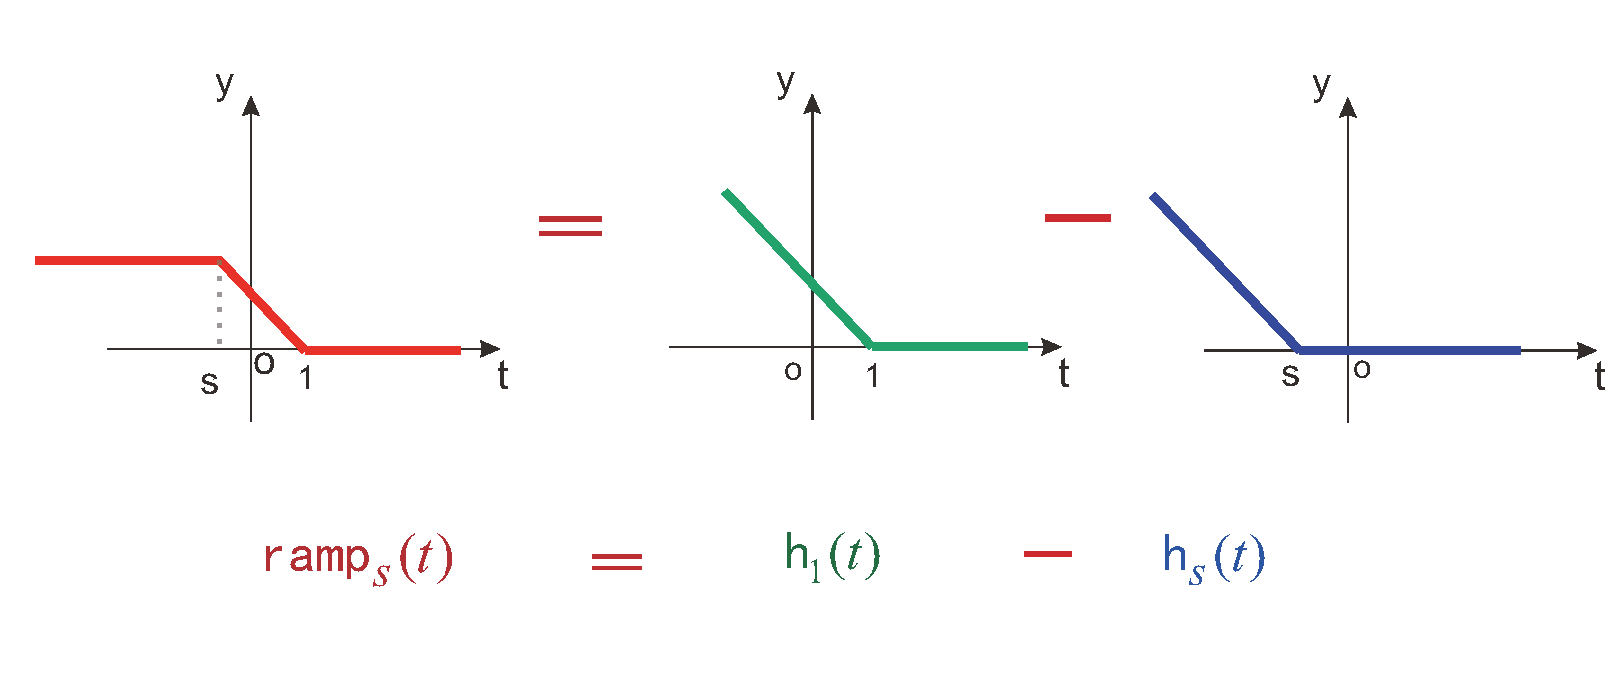
\includegraphics[width=0.9\textwidth]{./figure/ramp}

其中$\textnormal{ramp}_{s}^{} (t) = \min(1-s,\max(0,1-t))$,$s<1$为参数.


分解得到两个凸函数分别为:
$$h_s^{}(t) = \max(0,s-t),h_1{}(t)= \max(0,1-t).$$

% \begin{equation}\label{EQ_DC_prog}
%\min_{\beta}^{} \  J_{vex}(\beta) + J_{cav}(\beta)
%\end{equation}


\end{frame}







 \begin{frame}
   \frametitle{E.g.2  指数平方损失函数}

考虑指数平方损失函数:
  $$
\phi_{\gamma}(t) = 1 - e^{-\frac{t^2}{\gamma}}.
$$

%\begin{proposition}%\label{prop-dc-exp}
\onslide<2->{
DC分解:
    \begin{equation*}
       \phi_{\gamma}(t) =       [ \phi_{\gamma}(t) + v(t) ] - v(t),
    \end{equation*}
    其中 $  \phi_{\gamma}(t) + v(t)$ 也是凸函数.
    尝试可得函数$v(t) = e^{\frac{t^2}{\gamma}}$是满足条件的函数之一.
%\end{proposition}
}

\onslide<3->{
\begin{figure}[H]
\begin{center}
 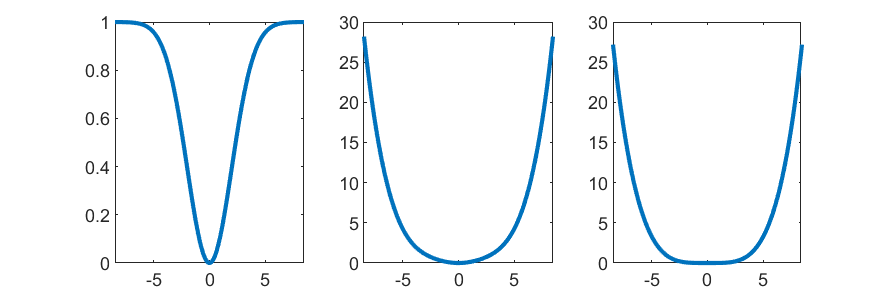
\includegraphics[width=0.7\textwidth]{figure/dc_exp_square}
\end{center}
\caption{左: 损失平方函数$\phi_{\gamma}(t)$; 中:  $\phi_{\gamma}(t) + v(t)$;
右:  $ v(t)$   }
\end{figure}
}

\end{frame}





%------------------------------------------
\begin{frame}
\frametitle{DC函数}
\begin{proposition}[命题]
令$f_{i}$,$i=1, \ldots m.$为DC函数,那么下列形式函数都属于DC函数。
\begin{enumerate}[(1)]
	\item $\sum_{i} \lambda_{i} f_{i}(x)$, for $\lambda_{i} \in \mathbb{R}$
	\item $\max _{i} f_{i}(x)$
	\item $\min _{i} f_{i}(x)$
	\item $\prod_{i} f_{i}(x)$
	\item  连续二阶可微函数$f$ 
 %$\Rightarrow$
	\item 如果函数$f$是$D C$函数,且函数$g$是凸函数, 那么复合函数$(g \circ f)$也是$D C$函数.
	%\item Every continuous function on a convex set %, $C$,
    %        is the limit of a sequence of uniformly converging DC functions.
    \item 凸集合上的每个连续函数都可以表示为一致收敛的DC函数的极限.
    % 凸集合上的每个连续函数都是一致收敛的DC函数的极限.
\end{enumerate}
\end{proposition}
\end{frame}



\section{DC规划和基本DC规划算法(DCA)}

\subsection{DC规划}
\begin{frame}
\frametitle{DC规划}

\begin{itemize}
  \item
   \hint{无约束DC规划}:
$$
\begin{array}{ll}
\underset{\mathbf{x} \in \mathbb{R}^{n}}{\operatorname{minimize}} & f_{0}(\mathbf{x}) \\
%\text { subject to } & f_{i}(\mathbf{x}) \leq 0, i=1, \ldots, m .
\end{array}
$$
$f_{0}: \mathbb{R}^{n} \rightarrow \mathbb{R}$是一个DC函数.


\item \hint{有约束DC规划:}
$$
\begin{array}{ll}
\underset{\mathbf{x} \in \mathbb{R}^{n}}{\operatorname{minimize}} & f_{0}(\mathbf{x}) \\
\text { subject to } & f_{i}(\mathbf{x}) \leq 0, i=1, \ldots, m .
\end{array}
$$
其中$f_{i}: \mathbb{R}^{n} \rightarrow \mathbb{R}$是DC函数,$i=0, \ldots, m$.



\end{itemize}

\end{frame}


\subsection{基本DC规划算法(DCA)}

\begin{frame}
\frametitle{基本DC规划算法(DCA)}

%\rule[-5pt]{14.3cm}{0.05em}
\noindent
\rule{0.9\textwidth}{0.05em}

\textbf{初始化:} 令 $x^{0} \in \operatorname{dom} \partial h, k=0 .$

\textbf{遍历} $k=0,1, \ldots$ 直到$\left\{x^{k}\right\}$ 收敛;%{until convergence of} $\left\{x^{k}\right\}:$\\
 
步1: 计算 $y^{k} \in \partial h\left(x^{k}\right)$;

步2: 计算
\begin{center}
\hint{$
x^{k+1} \in \operatorname{argmin}\left\{g(x)-h_{k}(x): x \in \mathbb{R}^{n}\right\} \quad \left(P_{k}\right)
$
 }
 \end{center}
\noindent
\rule[-1pt]{0.9\textwidth}{0.05em}

\begin{itemize}
  \item $h_{k}(x) = h(x^k)+\langle y^k,x-x^k\rangle $;
  \item $x\in \mathbb{R}^n \rightarrow x \in C $
\end{itemize}


\end{frame}
%------------------------------------------



\subsection{CCCP}
\begin{frame}
\frametitle{CCCP算法}

\normaltitle{CCCP是DCA在光滑优化中的一个示例.}

%The concave-convex procedure (CCCP) was first proposed for constructing discrete time dynamical systems that can be guaranteed to decrease almost any global optimization/energy function.\\

\begin{itemize}
  \item \dred{假设目标函数$f$是一个二阶可微函数}

  $\Rightarrow$ $f$是DC函数, $f(x) = f_{\text {vex }}(x)+  f_{\text {cav }}(x) $

  \item \dred{假设可行集是凸集C;} %defined by linear constraints

  \item CCCP算法每次迭代都\hint{用切线逼近凹函数},并极小化得到的凸函数:
%         and minimizes the resulting convex function
\end{itemize}
\hint{
$$
x^{k+1} \in \arg \min \left\{f_{v e x}(x)+\left\langle x, \dred{\nabla f_{c a v}(x^{k})}\right\rangle: x \in C\right\}
$$
}

\end{frame}
%--------------------------------------------
\begin{frame}
\frametitle{CCCP (Convex-Concave Procedure)}
%\textbf{CCCP algorithm} %-- \blue{Nonconvex problem $\rightarrow$ Convex problem}

$$\min _{x} \quad f_{\text {vex }}(x)+f_{\text {cav }}(x)$$
\onslide<2->{
\rule[-1pt]{0.95\textwidth}{0.05em}
\textbf{算法}  Concave-Convex procedure CCCP 对于求解$x$

\noindent
\rule[-1pt]{0.95\textwidth}{0.05em}

1: \textbf{初始化:} 令$x^{0}\in C $ ,$k=0$

2: \textbf{遍历} $k=0,1, \ldots$

3: $\quad x^{k+1}=\operatorname{argmin}_{x} f_{\text {vex }}(x)+\left\langle\nabla f_{\text {cav }}\left(x^{k}\right), x\right\rangle$

4: \textbf{直到} $\left\{x^{k}\right\}$ 收敛.

\noindent
\rule[-1pt]{0.95\textwidth}{0.05em}
}
%
%\onslide<3->{
%CCCP is nothing else than DCA for smooth optimization.
%}
\end{frame}
%--------------------------------------------------------
\begin{frame}
\frametitle{CCCP (Convex-Concave Procedure)}
对于\hint{凸函数 $g,h$: }
$$\min_x f(x) = g(x)-h(x)
$$
\begin{figure}
\centering
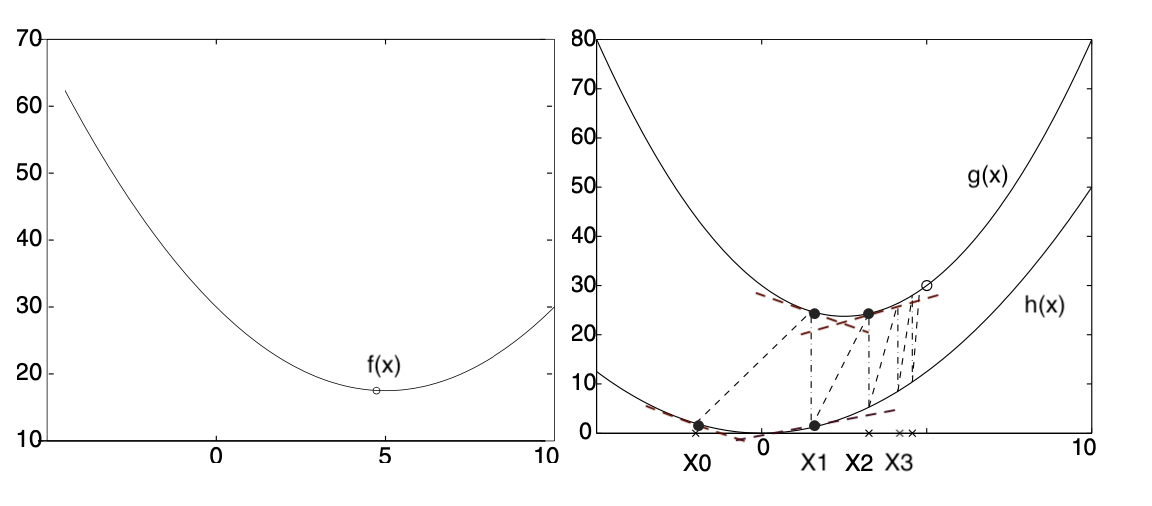
\includegraphics[width=0.8\textwidth]{picture/CCCP-algorithm.png}
\end{figure}
\begin{itemize}
\item<only@1-2> 当$ g,h \in \mathcal{C}^1$时  $\Rightarrow$ $f\in \mathcal{C}^1$;
\item<only@2> $x^*\in\text{argmin}_x f$  $\Rightarrow$ $\nabla f(x^*) = \nabla g(x^*) - \nabla h(x^*) = 0$;
\item<only@3-> 存在$x^{k+1}\in\text{argmin}_x [g(x)-h_k(x)]$
 \item<only@4->    $\Rightarrow$    寻找 $x^{k+1}$使得:     $\nabla g(x^{k+1}) - \nabla h(x^k) = 0$.

\end{itemize}


\end{frame}


\subsection{DCA性质}

\begin{frame}

\frametitle{DCA的性质}

%\rule[-5pt]{14.3cm}{0.05em}
\noindent
\rule{0.95\textwidth}{0.05em}

\textbf{初始化:} 令$x^{0} \in \operatorname{dom} \partial h, k=0 .$\\
\textbf{遍历} $k=0,1, \ldots$直到$\left\{x^{k}\right\}$ 收敛:\\ %\textbf{until convergence of} $\left\{x^{k}\right\}:$\\
step1: 计算 $y^{k} \in \partial h\left(x^{k}\right)$;\\
step2: 计算 \hint{$x^{k+1} \in \operatorname{argmin}\left\{g(x)-h_{k}(x): x \in \mathbb{R}^{n}\right\} \quad \left(P_{k}\right)$. }

\noindent
\rule[-1pt]{0.95\textwidth}{0.05em}
  \onslide<2->{

  \begin{itemize}
    \item 最优解集为$\left(P_{k}\right)$:  $\partial g^{*}\left(y^{k}\right)$
\item      DCA方法可以用另一种形式表示:%in another form:
$$
\begin{aligned}
\text{遍历} &\ k=0,1, \ldots\\
& \text{令}\quad y^{k} \in \partial h\left(x^{k}\right),
            \qquad x^{k+1} \in \partial g^{*}\left(y^{k}\right). \\
\end{aligned}
$$
  \end{itemize}

}


\end{frame}


\begin{frame}
\frametitle{DCA的性质}

\hint{DCA是一种无需线搜索的下降法,但具有全局收敛性.}

\begin{itemize}[<+->]
	%\item  $g\left(x^{k+1}\right)-h\left(x^{k+1}\right)=g\left(x^{k}\right)-h\left(x^{k}\right)$, then $x^{k}$ is a critical point of $g-h$. In this case, DCA terminates at $k$ th iteration.
	\item 如果问题的最优值α是有限的且无限序列$\left\{x^{k}\right\}$ 是有界的,则该序列的每一个极限点$x^{*}$都是$g-h$的一个临界点

	\item 对一般的DC规划,DCA具有线性收敛性.
	\item 在 \hint{多面体DC规划中} $\Rightarrow$ 序列$\left\{x^{k}\right\}$包含有限多个元素,经有限多次迭代后,DCA收敛到临界点$x^{*}$.
\end{itemize}
\end{frame}


\subsection{近似DCA}
%----------------------------------------------
\begin{frame}
\frametitle{近似DCA}

\begin{itemize}
  \item 基本的DCA方法:
  $y^{k} \in \partial h\left(x^{k}\right)$,
  $x^{k+1} \in \partial g^{*}\left(y^{k}\right) .$

\item
\hint{难点.}
 这些计算不一定都是准确的

  \item \hint{解决方法.}
使用近似DCA方法:
\hint{
 $$
 y^{k} \in \partial_{\varepsilon_{k}} h\left(x^{k}\right);
  \quad x^{k+1} \in \partial_{\varepsilon_{k}} g^{*}\left(y^{k}\right) .
 $$
 }
 \item
已经被证明:approximate DCA方法仍然收敛到一个临界点为$\varepsilon_{k} \downarrow 0$.

\end{itemize}

\end{frame}


%%===================================================

\section{应用}
\begin{frame}
  \frametitle{\secno\,\secname}
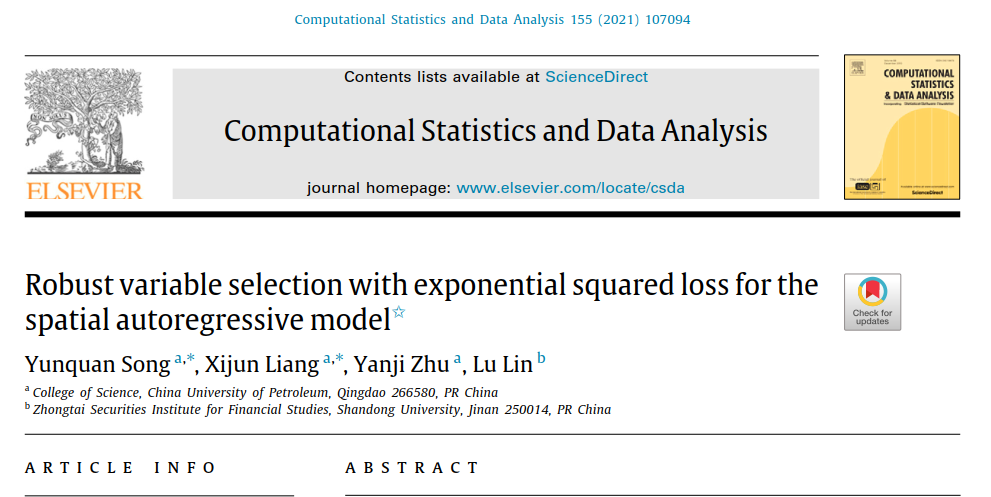
\includegraphics[width = 1.0\textwidth]{CSDA.png}

 \end{frame}


\begin{frame}
  \frametitle{\secno\,\secname}

考虑如下优化模型

\begin{equation}\label{eq-obj-L}
\min\limits_{\beta\in R^p,\rho\in [0,1]}^{} \quad L(\beta,\rho)=
  \frac{1}{n}\sum_{i=1}^n\phi_{\gamma}(Y_i - \rho \tilde{Y}_i - X_i\beta) + \lambda\sum_{j=1}^pP(|\beta_j|) %\eqno{(15)}
\end{equation}
其中$\lambda >0$, $\tilde{Y} = WY$, $\sum_{j=1}^p P(|\beta_j|)$ 惩罚项,
 $\phi_\gamma(\cdot)$ 是 \hint{指数平方损失函数:}
 $$\phi_\gamma(t)=1-\exp(-t^2/\gamma).
 $$

\end{frame}


\begin{frame}[fragile]

\begin{algorithm}[H]
\caption{The block coordinate descent (BCD) algorithm }
\label{alg-main}
%\algsetup{
%    linenosize=\small,
%    linenodelimiter=.
%}
%\setstretch{1.35}

\begin{algorithmic}[1]
\STATE     令初始值   $\beta^0 \in \mathbb{R}^{p}$且$\rho^0 \in (0,1) $;  %and $k=0$;
\STATE 遍历 $k = 0,1,2,\cdots$
\STATE %\label{step-rho-alg-main}
使用初始点 $\rho$ 对$\rho^k$进行迭代:
       \hint{\begin{equation} \label{eq-min-rho}
        \rho^{k+1}\leftarrow \min_{\rho\in [0,1]} L(\beta^{k},\rho );
     \end{equation}
     }
\STATE %\label{step-beta-alg-main}
 进一步更新 $ \beta^k$,通过
 \hint{
  \begin{equation} \label{eq-min-beta}
    \min_{\beta\in R^p} L(\beta ,\rho^{k+1})
     \end{equation}
}
可得到 $ \beta^{k+1}$, 需保证
    $L(\beta^{k},\rho^{k+1}) - L(\beta^{k+1},\rho^{k+1}) \leq 0$,且
    $\beta^{k+1}$在$L(\beta ,\rho^{k+1})$上是一个稳定点.

\STATE     令$k\leftarrow k+1$
\STATE{直到收敛. }

\end{algorithmic}
\end{algorithm}


\end{frame}



\begin{frame}
   \frametitle{E.g.2指数平方损失函数}

指数平方损失函数:
  $$
\phi_{\gamma}(t) = 1 - e^{-\frac{t^2}{\gamma}}.
$$


DC分解:
    \begin{equation*}
      \hint{ \phi_{\gamma}(t) =       [ \phi_{\gamma}(t) + v(t) ] - v(t),}
    \end{equation*}
    其中 $  \phi_{\gamma}(t) + v(t)$ 也是凸函数.
    尝试可得函数$v(t) = e^{\frac{t^2}{\gamma}}$是满足条件的函数之一.


\only<2>{
\begin{figure}[H]
\begin{center}
 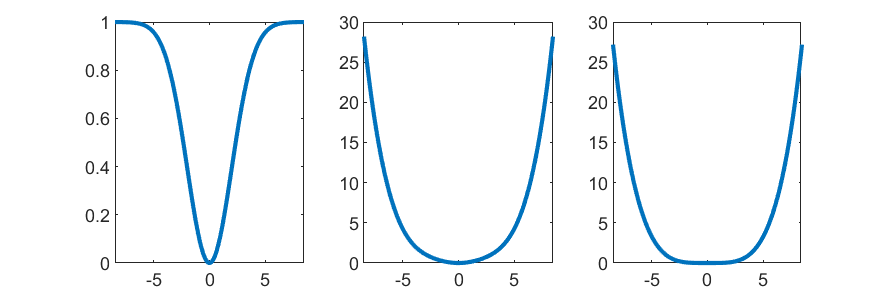
\includegraphics[width=0.7\textwidth]{figure/dc_exp_square}
\end{center}
\caption{左: 指数损失函数$\phi_{\gamma}(t)$; 中:  $\phi_{\gamma}(t) + v(t)$,
右:  $ v(t)$   }
\end{figure}
}


\only<3>{
 \dred{$e^{\frac{t^2}{\gamma}}$ 可能会引起计算困难:}
 当 $\gamma =1, t=10$, $e^{\frac{t^2}{\gamma}} = e^{100}\approx 2.688\times10^{43}$, 值过大$\rightarrow$ 计算缺陷.
}


\only<4->{
\begin{proposition}\label{prop-dc-exp}
    %The exponential squared loss function $\phi_{\gamma}(t)$ can be expressed as the difference of two convex functions:
    [另一种分解]
\begin{equation}\label{EQ-exp-sq-DC}
    \phi_{\gamma}(t) := [\phi_{\gamma}(t) + v(t)] - v(t) := u(t) - v(t),
\end{equation}

    $\dred{v(t) = \frac{1}{3\gamma^2}t^4}$, 
    $u(t) = \phi_{\gamma}(t) + v(t).$
\end{proposition}

}

\end{frame}


\begin{frame}

 \frametitle{目标函数的DC分解}

记:
  \begin{equation}\label{EQ_J_cav_J_vex}
\begin{array}{l}
J_{\textnormal{vex}}^{}(\beta)=  \frac{1}{n}\sum_{i=1}^n\ u(Y_i - \rho^k \langle w_i,Y\rangle - X_i\beta) + \lambda\sum_{j=1}^p P(|\beta_j|), \\
J_{\textnormal{cav}}^{}(\beta) = \frac{1}{n}\sum_{i=1}^n\ v(Y_i - \rho^k \langle w_i,Y\rangle - X_i\beta)  , \\
\end{array}
\end{equation}
 其中 %$u(\cdot)$, $v(\cdot)$ defined in (\ref{EQ-exp-sq-DC}),
  $w_i$是权重矩阵 $W$ 的第$i$行,
  $\sum_{j=1}^p\ P(|\beta_j|)$ 一个关于 $\beta$的凸惩罚项.

%Then, $J_{\textnormal{vex}}^{}(\cdot)$ and  $J_{\textnormal{cav}}^{}(\cdot)$
% are convex and concave functions respectively.

求解函数\,(\ref{eq-min-beta})% is formulated as
\begin{equation*}
  \min_{\beta\in R^p}^{} \quad  L(\beta,\rho^k) =
    J_{\textnormal{vex}}^{}(\beta) + J_{\textnormal{cav}}^{}(\beta),
\end{equation*}
$\longrightarrow$ 凹凸过程算法(CCCP) % framework %(\cite{CCCP2001}) %\cite{yuille2003}
%as shown in Algorithm\,\ref{Alg_general_CCCP}.  %% converges and works well,


\end{frame}


\begin{frame}%[fragile]

\begin{algorithm}[H]

\caption{The    Concave-Convex Procedure (CCCP)  } \label{Alg_general_CCCP}

\algsetup{
    linenosize=\small,
    linenodelimiter=.
}


\begin{algorithmic}[1]



\STATE     初始化 $\beta_{}^{0}$. 令$k=0$.

\REPEAT
\STATE     \begin{equation}\label{EQ_ite_CCCP}
        \beta_{}^{k+1} = \textnormal{argmin}_{\beta}^{} \quad J_{\textnormal{vex}}^{}(\beta) + J_{\textnormal{cav}}^{\prime}(\beta^k)\cdot \beta
     \end{equation}
\UNTIL{收敛至$\beta_{}^{k}$}.

 \end{algorithmic}
\end{algorithm}


\end{frame}



\begin{frame}[allowframebreaks]
  \frametitle{求解CCCP问题I}



\begin{itemize}
  \item
 $J_{\textnormal{cav}}^{\prime}(\beta^k)\cdot \beta$关于$\beta$是线性的,

 % have by the definition of
%$J_{\textnormal{vex}}^{}(\beta)$ in (\ref{EQ_J_cav_J_vex}) that
%the objective function
\item $J_{\textnormal{vex}}^{}(\beta) + J_{\textnormal{cav}}^{\prime}(\beta^k)\cdot \beta$ $\rightarrow$
\begin{equation}\label{EQ_f_plus_g}
  \min_{\beta\in R^p}\quad   \psi(\beta) + \lambda \sum_{i=1}^{p} P(|\beta_i|),
\end{equation}
其中$\psi(\beta)\in \mathcal{C}^1$是凸的,
 $  \sum_{i=1}^{p} P(|\beta_i|) $是Lasso惩罚项, %$  \sum_{i=1}^{p}  |\beta_i| $,
或者自适应Lasso惩罚项, $  \sum_{i=1}^{p} \eta_i |\beta_i| $, $\eta_i \geq 0$, $i=1,\cdots,p$.


\item
\cite{beck2009}: ISTA和FISTA算法,使用结构(\ref{EQ_f_plus_g})的 Lasso惩罚项求解了该模型.

\item  $\rightarrow$ (泛化): 使用自适应Lasso惩罚项求解该模型.
\end{itemize}
\end{frame}

\begin{frame}{求解CCCP问题II}
    

\begin{itemize}
  \item  ISTA 近似 $F(\beta)=\hint{\psi(\beta)} + \lambda\sum_{i=1}^{p} \eta_i |\beta_i|$ at $\beta = \xi$ as:
\begin{equation*}
  Q_{L}^{}(\beta,\xi) = \hint{\psi(\xi) + \langle \beta-\xi,\nabla \psi(\xi) \rangle  + \frac{L}{2}\|\beta-\xi\|_{}^{2} }
   +    \lambda\sum_{i=1}^{p} \eta_i |\beta_i|.
\end{equation*}

\item 这个函数拥有最小值点
\begin{equation}\label{EQ_P_L}
  \begin{aligned}
   \hint{ \Theta_{L}^{}(\xi)} & {=} \textnormal{argmin}_{\beta\in R^p}^{} \ Q_{L}^{}(\beta,\xi) \\
        & = \textnormal{argmin}_{\beta \in R^p}^{}\ \{   \lambda\sum_{i=1}^{p} \eta_i |\beta_i| + \frac{L}{2}\|\beta-(\xi-\frac{1}{L} \nabla \psi(\xi)\|_{}^{2} \} \\
        &  =  \mathcal{S}_{\lambda\eta/L}^{} (\xi - \frac{1}{L} \nabla \psi(\xi)),
  \end{aligned}
\end{equation}
\end{itemize}
\end{frame}


\begin{frame}{求解CCCP问题III}

其中$\eta = [\eta_1, \cdots, \eta_p]\in R^p$, 且有$\nu = \lambda\eta/L \in R_+^p$,
 $\mathcal{S}_{\alpha}^{}:\mathbb{R}_{}^{p} \rightarrow \mathbb{R}_{}^{p}$  软阈值算子
\begin{equation*}%\label{EQ_shrinkage_operator}
  \mathcal{S}_{\nu}(\beta) = \bar{\beta}, \quad \bar{\beta}_{i}^{} = (|\beta_{i}^{}|-\nu_i)_{+}^{} \sgn(\beta_{i}^{}), \ i=1,\ldots,p.
\end{equation*}
\begin{itemize}

\item  ISTA 求解 (\ref{EQ_f_plus_g}):
\begin{equation*}
  \beta_{}^{k} = \Theta_{L}^{}(\beta_{}^{k-1}).
\end{equation*}

\item 提升ISTA速度的变形 $\rightarrow$  FISTA


    \end{itemize}

\end{frame}



\begin{frame}
  \frametitle{求解$\rho$}

  \begin{itemize}
    \item
       \begin{equation} \label{eq-min-rho}
        \rho^{k+1}\leftarrow \min_{\rho\in [0,1]} L(\beta^{k},\rho );
     \end{equation}

  最小化一个单变量函数在区间[0,1]上 $\longrightarrow$
   经典的\hint{黄金分割搜索算法}% based on parabolic interpolation
% can be employed.

\item 比较模型\hint{相对应到平方损失:}
   \begin{equation}\label{eq_min_rho}
    \min_{\rho \in (0,1)}^{} L(\rho,\beta^k):= \frac{1}{n} \| y-X\beta^k - \rho W y\|_2^2 + \lambda \sum_{i=1}^p\  P(|\beta_i|).
 \end{equation}

 最优解:
\begin{equation}\label{eq-rho-sol}
    \rho^* = \textnormal{Proj}_{[0,1]}^{}\ \frac{\langle y-X\beta^k, W y\rangle }{\|Wy\|_2^2}
\end{equation}
其中
$
\textnormal{Proj}_{[0,1]}^{}(t) = \left\{\begin{array}{cl}
t, & t \in [0,1], \\
        1, & t> 1, \\
        0, & t<0.  \\
   \end{array}\right.
$
\end{itemize}

\end{frame}


\begin{frame}
\frametitle{实验}


\begin{figure}
%\begin{subfigure}{.65\textwidth}
  \centering

  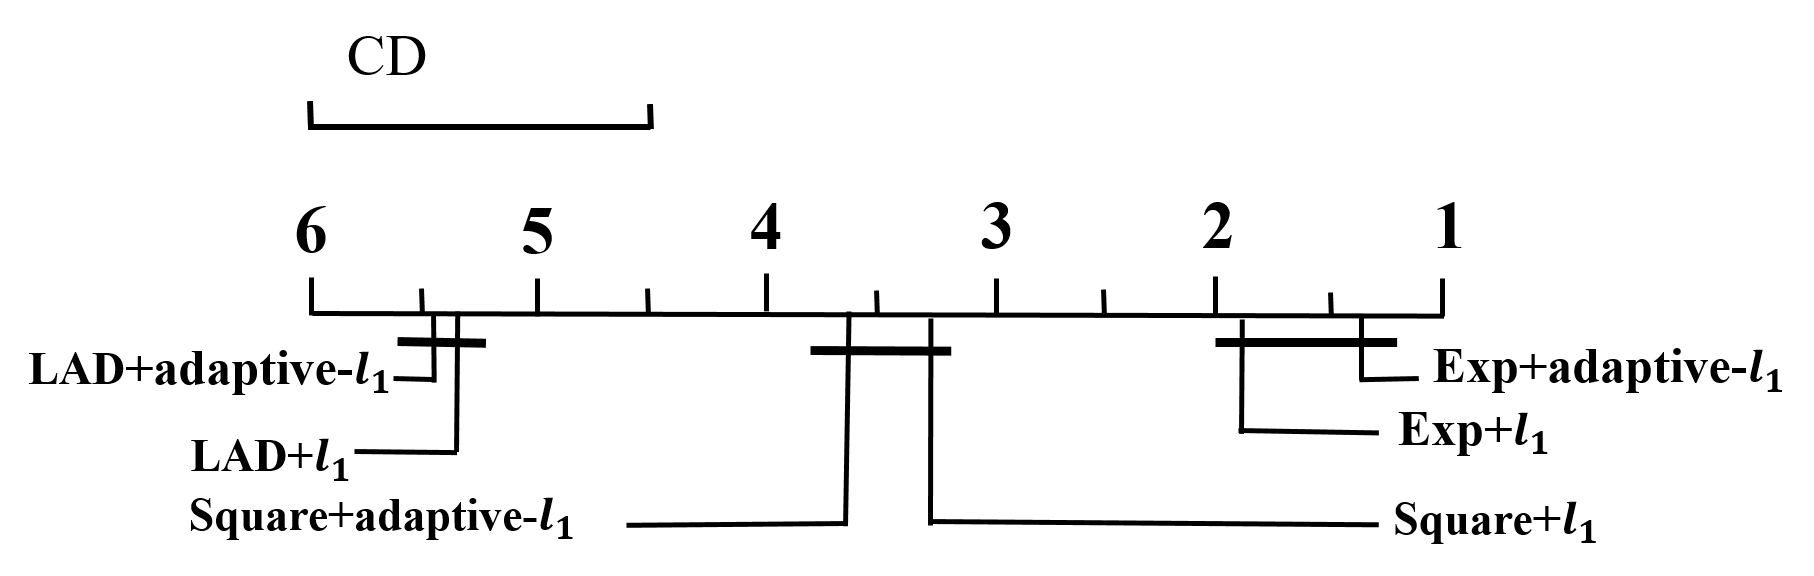
\includegraphics[width=.75\linewidth]{picture/stat-table7-correct}
  %\caption{ for ``Correct'' }%,   corresponding to Table\,\ref{tab-reg-outlier-y}.  }
  %\label{fig-correct-table7}
%\end{subfigure}
%\newline
\vspace{3ex}
%\begin{subfigure}{.65\textwidth}
%  \centering
  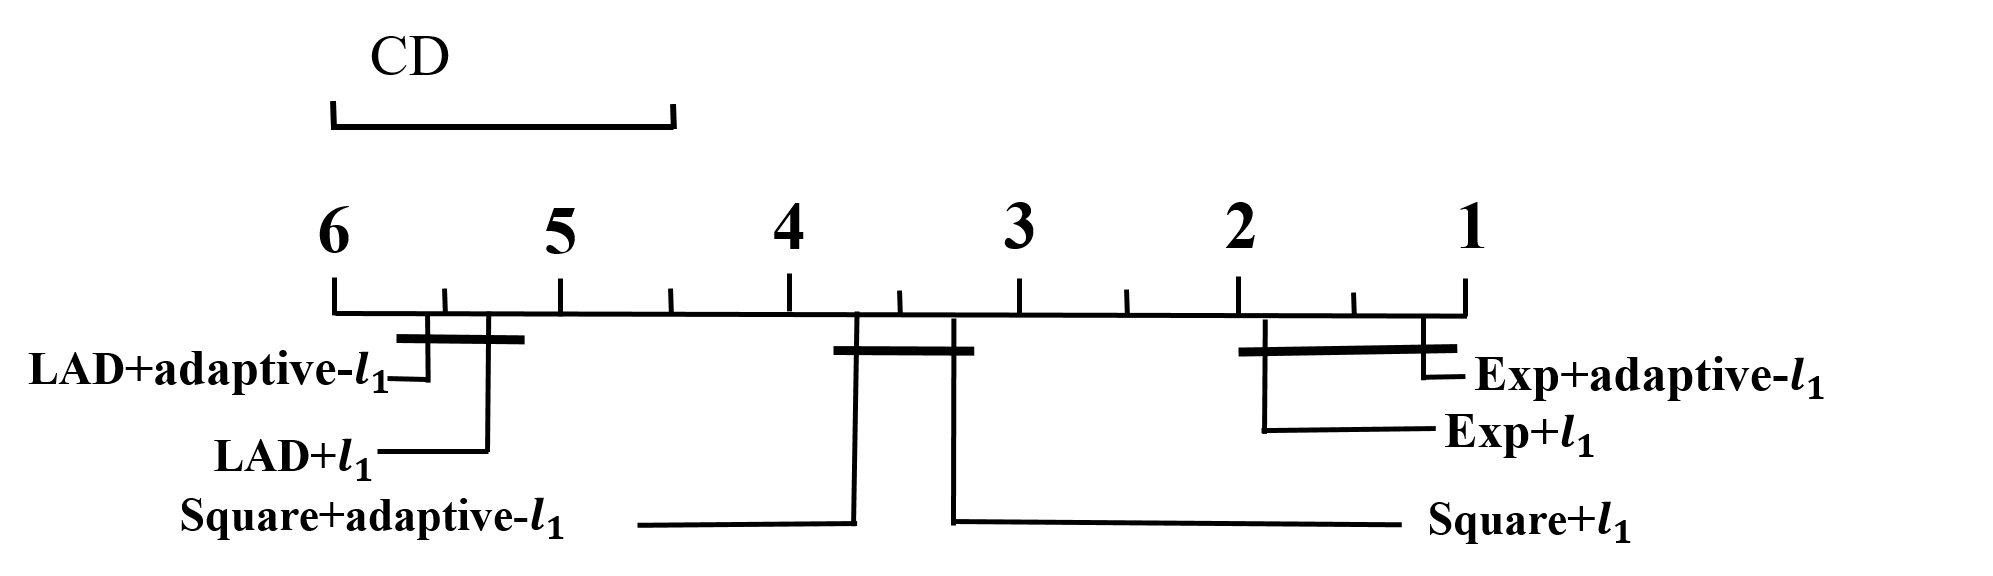
\includegraphics[width=.75\linewidth]{picture/stat-table7-MedSE}
%  \caption{ for ``MedSE'' }%,  corresponding to Table\,\ref{tab-reg-outlier-y}.  }
%  \label{fig-medse-table7}
%\end{subfigure}
\caption{Nemenyi test with regularizers with outliers in $y$, 置信水平: $\alpha=0.05$.
Top:  for ``Correct'' , Bottom: for ``MedSE''
 }
  \label{fig-stat-table7}
\end{figure}

\end{frame}



\begin{frame}

\bibliographystyle{plainnat}
  \bibliography{stat,opt,ref-homotopy,SAR}
  \end{frame}
\end{document}
